%texexptitled======================================================================
% lab1-gcd
%-----------------------------------------------------------------------
%

\documentclass[11pt]{article}

% Package includes

\usepackage[table]{xcolor}
\usepackage{graphicx}
\usepackage{color}
\usepackage{comment}
\usepackage{multirow}
\usepackage{askmaps}
\usepackage{karnaughmap}
\usepackage{amssymb}
\usepackage{amsmath}
\usepackage{gensymb}
\usepackage{arydshln}

% Wrap long URLs with hyphens
\PassOptionsToPackage{hyphens}{url}\usepackage{hyperref}
\usepackage[T1]{fontenc} %Get better tilde
\usepackage{lmodern} %Get better tilde
\usepackage{pdftexcmds}
\usepackage{pdfpages}
\usepackage{upquote}
\usepackage{textcomp}
\usepackage{minted}
%\usepackage[listings]{tcolorbox}
\usepackage{enumerate}
\usepackage{enumitem}
\usepackage{mathtools}
\usepackage{tikz}
\usepackage{circuitikz}
\usetikzlibrary{arrows, positioning, shapes.geometric, circuits.logic.US}
\tikzstyle{line}=[draw]
\tikzstyle{arrow}=[draw, -latex]
\usepackage[framemethod=tikz]{mdframed} %For easy shading of solutions

\usepackage{datetime2} % can get the time the PDF was generated
\usepackage{fancyhdr} % can set the footer


\usepackage{enumitem} % I'm not sure why I needed this
\usepackage[symbol]{footmisc} % use symbolic footnote symbols, except it doesn't work
\renewcommand{\thefootnote}{\fnsymbol{footnote}}

\DeclarePairedDelimiter{\ceil}{\Big\lceil}{\Big\rceil}

%\tcbset{
%texexp/.style={colframe=black, colback=lightgray!15,
%         coltitle=white,
%         fonttitle=\small\sffamily\bfseries, fontupper=\small, fontlower=\small},
%     example/.style 2 args={texexp,
%title={Question \thetcbcounter: #1},label={#2}},
%}
%
%\newtcolorbox{texexp}[1]{texexp}
%\newtcolorbox[auto counter]{texexptitled}[3][]{%
%example={#2}{#3},#1}

\setlength{\topmargin}{-0.5in}
\setlength{\textheight}{9in}
\setlength{\oddsidemargin}{0in}
\setlength{\evensidemargin}{0in}
\setlength{\textwidth}{6.5in}

% Useful macros

\newcommand{\note}[1]{{\bf [ NOTE: #1 ]}}
\newcommand{\fixme}[1]{{\bf [ FIXME: #1 ]}}
\newcommand{\wunits}[2]{\mbox{#1\,#2}}
\newcommand{\um}{\mbox{$\mu$m}}
\newcommand{\mm}{\mbox{mm}}
\newcommand{\nm}{\mbox{nm}}
\newcommand{\xum}[1]{\wunits{#1}{\um}}
\newcommand{\by}[2]{\mbox{#1$\times$#2}}
\newcommand{\byby}[3]{\mbox{#1$\times$#2$\times$#3}}
\usepackage{siunitx}

\newenvironment{tightlist}
{\begin{itemize}
 \setlength{\parsep}{0pt}
 \setlength{\itemsep}{-2pt}}
{\end{itemize}}

\newenvironment{titledtightlist}[1]
{\noindent
 ~~\textbf{#1}
 \begin{itemize}
 \setlength{\parsep}{0pt}
 \setlength{\itemsep}{-2pt}}
{\end{itemize}}

% Change spacing before and after section headers

\makeatletter
\renewcommand{\section}
{\@startsection {section}{1}{0pt}
 {-2ex}
 {1ex}
 {\bfseries\Large}}
\makeatother

\makeatletter
\renewcommand{\subsection}
{\@startsection {subsection}{1}{0pt}
 {-1ex}
 {0.5ex}
 {\bfseries\normalsize}}
\makeatother

% Reduce likelihood of a single line at the top/bottom of page

\clubpenalty=2000
\widowpenalty=2000

% Other commands and parameters

\pagestyle{fancy}
\setlength{\parindent}{0in}
\setlength{\parskip}{10pt}

% Commands for register format figures.

\newcommand{\instbit}[1]{\mbox{\scriptsize #1}}
\newcommand{\instbitrange}[2]{\instbit{#1} \hfill \instbit{#2}}

\newif\ifsolution
\newenvironment{solution}
%{\begin{mdframed}[backgroundcolor=gray!10, frametitle={Solution:}, frametitlebackgroundcolor=black, frametitlefont={\color{white}}]} %see http://mirror.utexas.edu/ctan/macros/latex/contrib/mdframed/mdframed.pdf
{\begin{mdframed}[frametitle={Solution:}, frametitlebackgroundcolor=black, frametitlefont={\color{white}}]} 
{\end{mdframed}}
%    {\color{red}}
%    {\color{black}}

\graphicspath{{./figs/}}

%Setting the fancy header & footer
\lhead{\assignmentname}
\rhead{\thepage}
\cfoot{\versionstamp}

%Display the version stamp on the 1st page but do not display the header
\fancypagestyle{plain}{%
\fancyhf{} % clear all header and footer fields
\fancyfoot[C]{\versionstamp} % except the center
\renewcommand{\headrulewidth}{0pt}
}

%Creating Column types for Fixed width (based on https://tex.stackexchange.com/questions/12703/how-to-create-fixed-width-table-columns-with-text-raggedright-centered-raggedlef)
\newcolumntype{L}[1]{>{\raggedright\let\newline\\\arraybackslash\hspace{0pt}}m{#1}}
\newcolumntype{C}[1]{>{\centering\let\newline\\\arraybackslash\hspace{0pt}}m{#1}}
\newcolumntype{R}[1]{>{\raggedleft\let\newline\\\arraybackslash\hspace{0pt}}m{#1}}

%Change Section Title Format (from https://tex.stackexchange.com/questions/245089/how-to-change-the-section-title-and-its-arrangement-in-a-latex-document)
%\renewcommand{\thesection}{\Roman{section}}
\usepackage{titlesec}
\titleformat{\section}
{\normalfont\Large\bfseries}{Problem~\thesection:}{1ex}{}

%-----------------------------------------------------------------------
% Document
%-----------------------------------------------------------------------


\begin{document}
\def\PYZsq{\textquotesingle}

\newcommand{\assignmentname}{EECS 151/251A Homework 1}
\newcommand{\versionstamp}{Version: 1 - \DTMnow}

\title{\vspace{-0.4in}\Large \bf \assignmentname \vspace{-0.1in}}
\author{Due Friday, September 9\textsuperscript{th}, 2022 11:59PM}

\date{}
\maketitle

\thispagestyle{plain}

\section*{Problem 1: Dennard Scaling}
Assuming perfect Dennard Scaling. Imagine a processor that runs at 5MHz \& 1A and dissipates 5W.
\begin{enumerate}[label=(\alph*)]
\item What would the power and performance be in the next technology node if transistors are 1.25x smaller? Remember units!

\item Show that power density is constant between the old and new technology node.

\end{enumerate}

\begin{solution}
\begin{enumerate}[label=(\alph*)]

\item $\kappa = 1.25$

New power $\dot P = P \frac{1}{\kappa^2} = 5 \frac{1}{1.25^2} =  \SI{3.2}{\watt}$ 

New capacitance $\dot C = C \frac{1}{\kappa}$ and new voltage $\dot V = V \frac{1}{\kappa}$

We know that $P = \frac{1}{2}C V^2f$ and s0:

$\dot P = P \frac{1}{\kappa^2} = \frac{1}{2}CV \frac{1}{\kappa^2} $

$=\frac{1}{2} \kappa \dot C \kappa^2 \dot V^2f\frac{1}{\kappa^2}$

$= \frac{1}{2} \dot C \dot V^2 (\kappa f)$

Thus new frequency $\dot f = \kappa f = 1.25 \cdot 5 = 6.25 = $ 6.25MHz

\item Power density is $\frac{V I}{A}$

We know that new voltage $\dot V = V \frac{1}{\kappa}$, new current $\dot I = I \frac{1}{\kappa}$, new area $\dot A = \frac{A}{\kappa^2}$

New power density is $\frac{\dot V \dot I}{\dot A} = \frac{V \frac{1}{\kappa} I \frac{1}{\kappa}}{\frac{A}{\kappa^2}} = \frac{V I}{A}$
\end{enumerate}

\end{solution}

\section*{Problem 2: What's that Circuit!}
\begin{enumerate}[label=(\alph*)]


\begin{figure}[H]
\centering
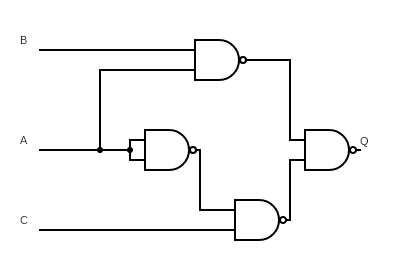
\includegraphics[width=0.6\textwidth]{figs/mux.png}
\caption{Circuit 1 for parts (a) (b) (c)}
\end{figure}

\item Write out and simplify the Boolean expression for circuit 1.
\item Write out the full truth table for circuit 1 based on the Boolean expression you found in part (a).
\item What is circuit 1 called?

\begin{solution}
\begin{enumerate}[label=(\alph*)]
\item  $\overline{(\overline{AB}) (\overline{\overline{A}C})}$

$AB + \overline{A}C$

\item   Truth Table \begin{center}
    \begin{tabular}{c c c | c}
    B  & C  & A & Q \\ \hline
    0  & 0  & 0 & 0\\ 
    1  & 1  & 0 & 1\\
    0  & 1  & 1 & 0\\
    1  & 0  & 1 & 1\\
    \end{tabular}
    \end{center}
\item   This is a MUX!
\end{enumerate}
\end{solution}

\begin{figure}[H]
\centering
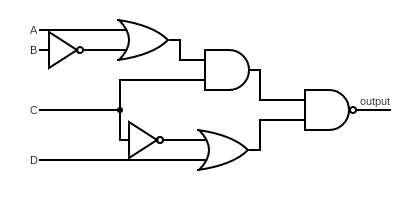
\includegraphics[width=0.6\textwidth]{figs/circuit.png}
\caption{Circuit 2 for parts (d) (e)}
\end{figure}

\item Write out and simplify the Boolean expression for circuit 2.
\item Write out the full truth table for circuit 2 based on the Boolean expression you found in part (d).

\end{enumerate}

\begin{solution}
\begin{enumerate}[label=(\alph*)]
\item  $\overline{(A + \overline{B})C(\overline{C}+D)}$

$\overline{A + \overline{B}} + \overline{C} + \overline{\overline{C} + D }$

$\overline{A}B + C + C \overline{D}$

$\overline{A}B + C(1 + \overline{D})$

$\overline{A}B + C$


\item   Truth Table \begin{center}
    \begin{tabular}{c c c c | c}
    A & B & C & D & output\\ \hline
    0 & 0 & 0 & 0 & 0\\ 
    1 & 0 & 0 & 0 & 0 \\
    0 & 1 & 0 & 0 & 1 \\ 
    1 & 1 & 0 & 0 & 0 \\
    0 & 0 & 1 & 0 & 1\\ 
    1 & 0 & 1 & 0 & 1 \\
    0 & 1 & 1 & 0 & 1 \\ 
    1 & 1 & 1 & 0 & 1 \\
    0 & 0 & 0 & 1 & 0\\ 
    1 & 0 & 0 & 1 & 0 \\
    0 & 1 & 0 & 1 & 0 \\ 
    1 & 1 & 0 & 1 & 0 \\
    0 & 0 & 1 & 1 & 1\\ 
    1 & 0 & 1 & 1 & 1 \\
    0 & 1 & 1 & 1 & 1 \\ 
    1 & 1 & 1 & 1 & 1 \\
    \end{tabular}
    \end{center}
\end{enumerate}
\end{solution}

\section*{Problem 3: Verilog}
For each example, identify the error in the Verilog code and suggest a fix. You don't have to rewrite the entire Verilog unless you think that's the most succinct \& clear way to answer.
\begin{enumerate}[label=(\alph*)]

\item \begin{minted}{verilog}
module example_one(
	input [1:0] a,
	input b, c,
	output x
);
	always @(*) begin
	    case (a)
	        2'b00 : x = b;
	        2'b01 : x = c;
	        2'b11 : x = b & c;
	        2'b10 : x = b | c;
	    endcase
	end
endmodule
\end{minted}

\begin{solution}
output x should be reg x. x is being assigned within an always block. 
\end{solution}

\item \begin{minted}{verilog}
module example_two(
	input a, b, c,
	output reg [1:0] x
);
    always @(*) begin
    	if (a & b & c) begin
    		x = 3;
    	end
    	else if (a & b) begin
    		x = 2;
    	end
    	else if (c) begin
    		x = 1;
    	end
    end
endmodule
\end{minted}

\begin{solution}
Include an else case to catch all other cases or exhaust all 8 cases possible with a,b, and c. Don't want to accidentally create a latch.
\end{solution}

\item \begin{minted}{verilog}
module example_three(
	input [1:0] a,
	input toggle, sel, 
	output reg x
);
    always @(toggle) begin
        if (sel) begin
            x = a[1];
        end
        else if (!sel) begin
    	x = a[0];
        end
    end
endmodule
\end{minted}

\begin{solution}
always @(toggle) should be either always @(*) or always @(toggle, sel, a)
\end{solution}

\end{enumerate}
\section*{Problem 4: Circuit Drawing! (251 Only)}
Draw a circuit that can realize any arbitrary 2 input function of signals A and B. 

\end{document}